\begin{figure}[h]
    \centering
    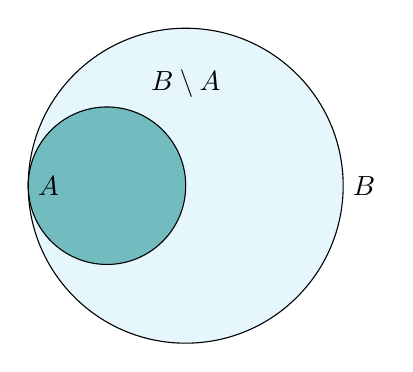
\begin{tikzpicture}
        \def\bigcircle{(1, 0) circle (2cm)}
        \def\smallcircle{(0, 0) circle (1cm)}
        \fill[cyan, fill opacity=0.1] \bigcircle;
        \fill[teal, fill opacity=0.5] \smallcircle;
        \draw \smallcircle;
        \draw \bigcircle;
        
        \node[right] at (-1, 0) {$A$};
        \node[right] at (3, 0) {$B$};
        \node[above] at (1, 1) {$B \setminus A$};
     \end{tikzpicture}
    \caption{Venn diagram of the event sets $A$ and $B$}
    \label{fig:venn}
\end{figure}
